\chapter{Dealing with File Bloat}\label{ch:bloat}

\section{Rationale}
In the system thus far described, the emphasis has been firmly upon reducing the computational complexity of layout operations at document view-time, and therefore little consideration has been given to the filesize of the output malleable documents.

%\todo{Put in some pdfdump output comparing ``normal'' pdfs with my malleable ones (maybe as an appendix)}

The tradeoff between filesize and required computation has previously been justified on the basis that storage is cheap,\marginpar{as of 2013 one US dollar will buy around two gigabytes of \textsc{nand} flash memory} light, and small, and that batteries, although relatively inexpensive, already comprise a significant proportion of the overall mass and volume of most portable devices suitable for reading \ebook{}s. The consequence of this is that adding more storage would have little impact upon devices' aesthetics, but adding extra battery life (emerging nanotube battery technology notwithstanding) would result in vast increases in devices' overall bulk and mass.

Despite this, it seems perverse to make no attempt at all to keep filesizes as small as possible, as long as there are no (or limited) impacts upon the required computation at view-time.

Much like typesetting algorithms, few compression algorithms are designed with the minimisation of computation in mind. Consequently, the result of compressing the data using some generic algorithm is likely to require significantly more computation to decompress than a carefully designed bespoke algorithm. The following section describes describes work towards such an algorithm.


\section{Implementation}
The most obvious saving that can be made is with the duplication of a document's textual content. The systems described in Chapters \ref{ch:malleable}~and~\ref{ch:floats} both contain as many copies of the document text as there are pre-rendered galleys. In practice, there is no real need for more than one copy to be present in the file. Two approaches to this problem were considered.

\subsection{Pointers into the Source Text}
The first approach to be considered was to include the source text of the document in its entirety, and for each rendering to contain only pointers to the relevant sections of text, instead of the words themselves. These pointers can either be absolute (in the form of a character offset from the start of the text) or logical (in the form \emph{paragraph m, word n}). If the document text is to be included as a plaintext string, absolute pointers are easier to use than logical: logical pointers either require an auxiliary data structure to map the logical pointers to absolute ones, or for the document text to be stored in a format reflecting the logical structure, \ie{} not in plain text.

The principle drawback of using this approach is that on occasion, the output of the linebreaking process does not precisely match the input: for example in the case where words are hyphenated (requiring one word to be broken into two parts, and the addition of a hyphen) or where certain glyphs may be substituted for others (such as with the use of ligatures, where a glyph pair or triplet may be replaced with a single glyph). For this reason, this approach was not considered further.


\subsection{Use of a Dictionary}
\label{sec:dictionary}
The second approach considered was the use of a dictionary to act as a lookup table for each word-level item produced by the linebreaking process.

A document's source text itself is likely to contain significant redundancy. In the 1930s, American linguist George Kingsley Zipf proposed \emph{Zipf's law}~\cite{zipf1932}, which (broadly) states that given a sizeable sample of text in any given language, the frequency of any word is inversely proportional to its rank in the frequency table. Stated another way, the most common word tends to appear twice as often as the second most common word, three times as often as the third most common word, and so on.

\begin{table} \footnotesize
    \myfloatalign
  \begin{tabularx}{\textwidth}{rrlrlrlrl} \toprule
    & \multicolumn{2}{l}{\textsc{Butterley}} & \multicolumn{2}{l}{\cite{Pinkney2011}} & \multicolumn{2}{l}{\textsc{Shakespeare}} & \multicolumn{2}{l}{\textsc{KJV}}\\
    \midrule
    & 103 & the & 233 & the & 23197 & the & 62099 & the \\ 
    & 35 & of & 134 & of & 19540 & I & 38576 & and \\ 
    & 33 & and & 116 & to & 18263 & and & 34445 & of \\ 
    & 31 & in & 75 & and & 15592 & to & 13387 & to \\ 
    & 25 & to & 75 & a & 15507 & of & 12735 & And \\ 
    & 23 & for & 56 & is & 12516 & a & 12451 & that \\ 
    & 23 & a & 52 & be & 10825 & my & 12167 & in \\ 
    & 21 & was & 50 & in & 9565 & in & 9760 & shall \\ 
    & 19 & company & 34 & as & 9059 & you & 9508 & he \\ 
    & 17 & Butterley & 32 & document & 7831 & is & 8932 & unto \\ 
    \midrule
    \textsc{total} & \multicolumn{2}{l}{1232} & \multicolumn{2}{l}{3724} & \multicolumn{2}{l}{899595} & \multicolumn{2}{l}{821133} \\ 
    \midrule
    \textsc{unique} & \multicolumn{2}{l}{628} & \multicolumn{2}{l}{1436} & \multicolumn{2}{l}{67107} & \multicolumn{2}{l}{33446} \\ 
    \bottomrule
    
  \end{tabularx}
  \caption[Word frequencies in various documents]{Top 10 most frequent words in various documents. The total number of words and total unique words are also shown for each document. The data used to produce this table assumes a word is considered to be any contiguous block of (case-sensitive) non-whitespace characters; thus, ``\texttt{\textcolor{red}{and}}'' is distinct from ``\texttt{\textcolor{red}{And}}'', and ``\texttt{\textcolor{red}{document}}'' is distinct from ``\texttt{\textcolor{red}{document.}}''. The rationale behind this is that the data produced is more closely representative of a real dictionary of atomic ``words'' to be typeset in a malleable document.}
  \label{tab:wordfreq}
\end{table}

\begin{figure}
  \begin{center}
  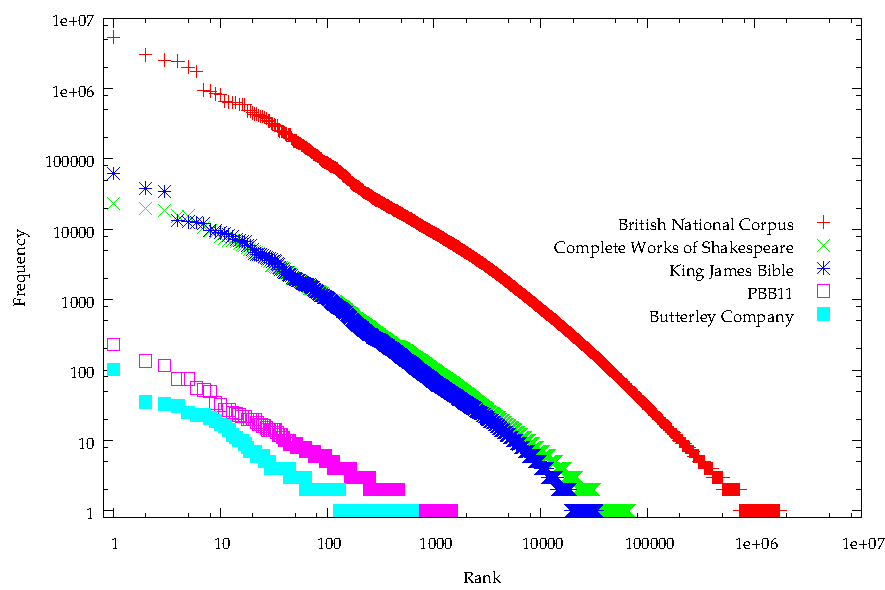
\includegraphics[width=\textwidth]{gnuplot/wordfreq}
  \end{center}
  \caption[Word frequencies in various documents]{Word frequencies in various documents, plotted on a log-log scale. All of these documents, despite their varying lengths, appear to conform well with Zipf's Law.}
  \label{fig:wordfreq}
\end{figure}

Table~\ref{tab:wordfreq} shows the ten most frequent words in four separate documents: the Wikipedia page for the \emph{Butterley Company}\footnote{\texttt{http://en.wikipedia.org/wiki/Butterley\_Company}}, the author's 2011 paper \emph{Reflowable Documents Composed from Pre-rendered Atomic Components} \cite{Pinkney2011}, the Complete Works of Shakespeare, and the King James Version of the Bible. Figure~\ref{fig:wordfreq} shows the complete frequency data for the same documents plotted on a log-log scale. At the extremities, the data does not conform perfectly to Zipf's Law, though despite their hugely varying lengths, each document does display a clear Zipfian distribution.

\begin{figure}
  \begin{center}
  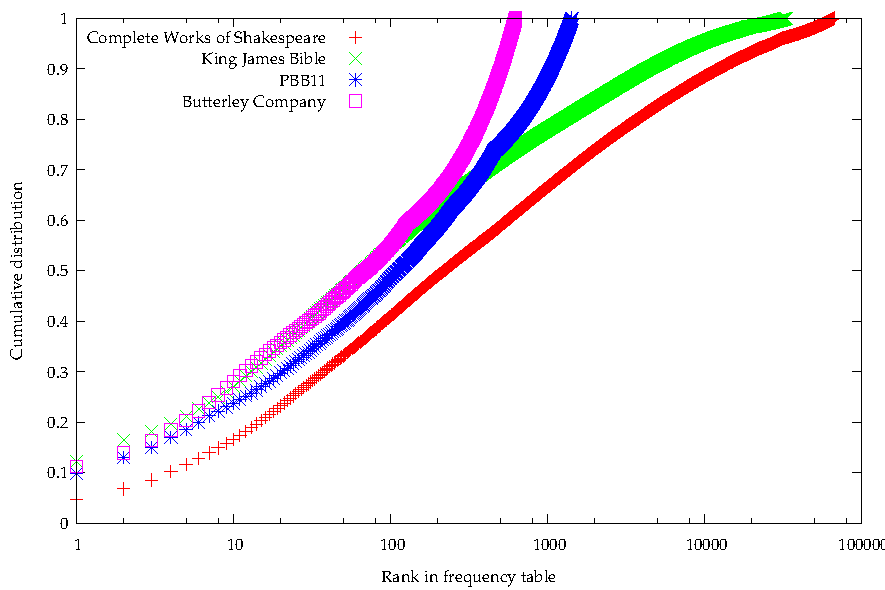
\includegraphics[width=\textwidth]{gnuplot/cumulative}
  \end{center}
  \caption[Cumulative distribution of word frequencies]{Cumulative distribution of word frequencies in various documents. (The x-axis uses a logarithmic scale so that the data for the two shorter documents is more clearly visible.)}
  \label{fig:cumulative}
\end{figure}

This inherent redundancy in natural language can be exploited to produce a simple compression scheme through use of a dictionary. If, for example, if the word ``shall'' appears multiple times in a document (in the King James Version of the Bible it appears 9760 times, and in the complete works of Shakespeare 3016 times) it is only stored once in the dictionary. As long as on average (\ie{} over every occurrence of every word) each word's key is lexicographically shorter than the word itself, it can be guaranteed that some redundancy has been removed from the data.

The \textsc{html} and \textsc{JavaScript} system described in Chapter~\ref{ch:floats} can be altered to use a dictionary-based lookup table with fairly few modifications. Firstly, since the data for the malleable document must be represented in \gls{json}, some means of including the dictionary must be devised. \gls{json} supports two types of collection: the first is the \emph{object}, which is defined formally as \emph{an \mbox{unordered} set of name/value pairs}. This acts much like an associative array, though there is no guarantee of order of elements.  The second collection type supported by \gls{json} is the \emph{array}, defined as \emph{an ordered collection of values}. Since both must be declared literally (in the forms \texttt{\{\textquotedbl key1\textquotedbl:\textquotedbl word1\textquotedbl,\textquotedbl key2\textquotedbl:\textquotedbl word2\textquotedbl\}} and \texttt{[\textquotedbl word1\textquotedbl,\textquotedbl word2\textquotedbl]} respectively\ed see \texttt{http://www.json.org/} for full details) rather than being populated programatically, using a plain array for the dictionary allows us to omit the keys from the dictionary itself, as they are implied by the order of the elements in the array. Additionally, since this forces the use of integers as keys, the Galley Structure Tree will not require the use of quote marks when the dictionary keys are referenced. If the keys were string values, each use of each key in the Galley Structure Tree would therefore necessitate two extra characters (\eg{} \texttt{\textquotedbl key\textquotedbl} versus \texttt{401}).

It should also be noted that using integers as keys in \gls{json} has different implications to using integers as keys in some more compact binary format. Data in \gls{json} is always stored in some textual encoding (perhaps \textsc{ascii}, perhaps \textsc{utf-8}), and there is no support for numeric representation in any base other than decimal. What might take up one 32 bit integer (\ie{} 4 bytes) in a compiled language such as \textsc{c} might take as many as ten textual characters (10 bytes, assuming that whichever character encoding system is used represents low-\textsc{ascii} characters with only one byte). Conversely, textual representation of integers can be more compact under certain conditions: namely, for values that use three or fewer characters, \ie{} the numbers 0--999.

Referring back to Figures \ref{fig:wordfreq}~and~\ref{fig:cumulative}, and to Zipf's law, it can be seen that even for extremely long documents, the number of words that occur are ranked in the top 1000 exceeds 60\%, and so in fact, as long as the order of words in the dictionary is chosen carefully, using a textual representation of integers can be more compact than a na\"ive binary representation.

It was therefore decided to store the dictionary as an array, ordered so that the most frequently occurring words have the smallest keys.

\newpage
\subsection{Further Compression Possibilities}
\label{sec:deltas}

The techniques discussed thus far have focused mostly upon exploiting the inherent redundancy in natural language (specifically redundancy in written English, though some non-rigorous research suggests this is also true in many other written languages). A fairly large part of the data contained within the Galley Structure Tree has been overlooked: the typesetting data itself.

All of the aforementioned encoding systems have used an absolute value for the positioning of each word on each line; that is, each occurrence of each word has an associated value representing the required distance of its placement, in \glspl{point}, from the start of the line. An example of this can be seen in Listing~\ref{lst:datajs} on page~\pageref{lst:datajs}.

With a vague view to producing data that would be more easily compressible by a generic compression algorithm (that would perhaps be useful if HTTP compression or similar is used to transfer the document data to a device) it was decided to investigate a different approach to storing this data.

In any typeset document, most (if not all) occurrences of the same word will be indistinguishable from one another. In particular, the amount of horizontal space a word uses will be consistent for each occurrence of the word. Similarly, if a document's text is fully justified, the space between words on each individual line will be identical. If the document is left-justified, then each space between each word on every line will be identical. This redundancy is present within all the previous encodings, but cannot be picked up by a generic compression algorithm, since it requires knowledge of the typesetting process. By separating the word widths from the spacing, this redundancy can be made more explicit, and therefore easier for a generic compression algorithm to take advantage of.

\begin{lstlisting}[label=lst:deltasdata,captionpos=b,float,language=c,stringstyle=\color{blue},basicstyle=\ttfamily\footnotesize,caption={[Excerpt from a paragraph tree using deltas]Excerpt from a JavaScript data file that uses position deltas in the Galley Structure Tree, representing one galley rendering of one paragraph.}]
[
    [[0,982],[3.678,26],[3.678,93],],
    [[0,14],[2.682,1307],[2.682,558],],
    [[0,7],[3.668,557],[3.668,797],[3.668,226],],
    [[0,102],[4.338,9],[4.338,30],],
    [[0,112],[2.4,1013],[2.4,1068],],
    [[0,182],[2.4,1303],[2.4,2],[2.4,547],],
    [[0,308],[15.666,15],[15.666,1114],],
    [[0,177],[2.4,1173],[2.4,229],[2.4,733],],
    [[0,19],[7.336,81],[7.336,26],[7.336,143],],
    [[0,96],[7.116,33],[7.116,97],[7.116,16],],
    [[0,141],[9.444,0],[9.444,30],[9.444,1],],
    [[0,0],[8.78,89],[8.78,8],[8.78,11],],
    [[0,905],[10.008,2],[10.008,0],[10.008,66],],
    [[0,1125],[5.922,5],[5.922,34],[5.922,0],[5.922,1172],],
    [[0,1],[2.676,1053],[2.676,471],],
    [[0,3],[4.008,967],[4.008,112],],
    [[0,524],[10.338,19],[10.338,0],],
    [[0,126],[7.356,571],[7.356,1],],
    [[0,0],[6.896,197],[6.896,16],[6.896,18],],
    [[0,0],[2.4,9],[2.4,5],[2.4,691],],
    [[0,1249],[14.004,1046],[14.004,317],],
    [[0,5],[11.112,289],[11.112,2],[11.112,0],],
    [[0,273],[9.84,24],[9.84,859],],
    [[0,986],[11.34,144],[11.34,210],],
    [[0,263],[2.4,774],],
],
\end{lstlisting}

\begin{lstlisting}[label=lst:deltasdict,captionpos=b,float,language=c,stringstyle=\color{blue},basicstyle=\ttfamily\footnotesize,caption={[Excerpt from a dictionary storing word widths]Excerpt from the dictionary from a JavaScript data file that uses position deltas, where the width of each word is stored alongside the word itself.}]
 [["the",14.664],["of",9.996],["to",9.336],["and",17.328],["a",5.328],["is",8.004],["be",11.328],["in",9.336],["as",9.996],["document",47.328],["that",18],["it",6.672],["page",22.656],["for",13.992],["are",14.652],["by",12],["on",12],["will",18.672],["which",29.328],["with",21.336],["this",17.34],["The",18.66],["can",16.656],["an",11.328],["or",9.996],["-",3.996],["eBook",31.332],["used",21.996],["PDF",22.008],["In",9.996],["layout",30],["have",22.656],["from",23.328],["not",15.336],["at",8.664],["width",27.336],["This",21.336],["has",15.996],["then",20.664],["each",21.984],["was",18.66],["typesetting",52.668],["columns",40.668],["simply",32.676],["these",24.66],["text",18],["into",18.672],["hyphenation",59.328],["content",35.328],["quality",33.336],["column",36],["lines",22.668],["only",21.336],["line",18],["ACM",27.336],["our",15.996],["its",11.34],["structure",41.988],["Document",49.992],["penalty",35.328],["between",39.984],["galley",29.328],["order",25.32],["more",24.66],["COGs",30],["out",15.336],["end",17.328],["one",17.328],["use",15.996],["algorithm",46.668],["producing",48.66],["columns.",43.668],["galleys",33.996],["figure",28.656],["simple",32.004],["would",30],
\end{lstlisting}

On the basis of the above observations, the decision was taken that the dictionary should be modified to store the width of each word alongside itself, and that the Galley Structure Tree should be modified so that each word to be typeset is now accompanied by the offset required from the end of the previous word (which shall henceforth be referred to as \emph{deltas}) rather than the absolute offset required from the start of the line. This does of course necessitate two array lookups in the dictionary where previously there would have been only one, but since array accesses run in constant time, it does not present too much of a problem. Excerpts from a Galley Structure Tree and dictionary that use this encoding system are shown in Listings \ref{lst:deltasdata}~and~\ref{lst:deltasdict} respectively.

Further redundancy could be removed by exploiting the fact that words tend to be regularly spaced on each line. Whilst the encoding could be modified to allow only regular spacing of words, it was felt that this might be somewhat restrictive, and would detract from the appeal of the system as something that supports complex, arbitrary layouts.

Even without making further compression attempts beyond the encoding system shown in Listings \ref{lst:deltasdata}~and~\ref{lst:deltasdict}\ed the motivation for which, we must remember, was to produce an encoding that was more \emph{compressible}, rather than more \emph{compressed}\ed by pure chance, it turns out that even in its full form, this is the most compact representation yet devised!



\newpage
\section{Results}

The following pages show the evolution of the encoding system, and how the filesizes vary according to the number of included galley renderings, for the same sample documents that are used for Figures \ref{fig:wordfreq}~and~\ref{fig:cumulative}:

\begin{itemize}

 \item Figure~\ref{fig:size-json} (page~\pageref{fig:size-json}) shows the ``original'' encoding system described in Chapter~\ref{ch:floats}, which does not make any attempt to minimise filesize.

 \item Figure~\ref{fig:size-unord} (page~\pageref{fig:size-unord}) shows the encoding system described in Section~\ref{sec:dictionary}, using a dictionary ordered such that the first occurring words have the shortest keys. (The dictionary is therefore described as \emph{unordered}.)

 \item Figure~\ref{fig:size-ord} (page~\pageref{fig:size-ord}) shows the encoding system described in Section~\ref{sec:dictionary}, using a dictionary ordered such that the most frequently occurring words have the shortest keys. (The dictionary is therefore described as \emph{ordered}.)

 \item Figure~\ref{fig:size-deltas} (page~\pageref{fig:size-deltas}) shows the encoding system described in Section~\ref{sec:deltas}, which not only uses a dictionary ordered such that the most frequently occurring words have the shortest keys, but also stores in the dictionary the width of each word, so that the Galley Structure Tree contains deltas rather than absolute positioning data.
 
 \item Figure~\ref{fig:size-all-b} on page~\pageref{fig:size-all-b} shows a comparison of the filesizes produced by all encodings. Figure~\ref{fig:size-all-gz} on page~\pageref{fig:size-all-gz} shows the resultant filesizes when each rendering is further compressed with \texttt{gzip}.
\end{itemize}



\begin{figure}
  \begin{center}
  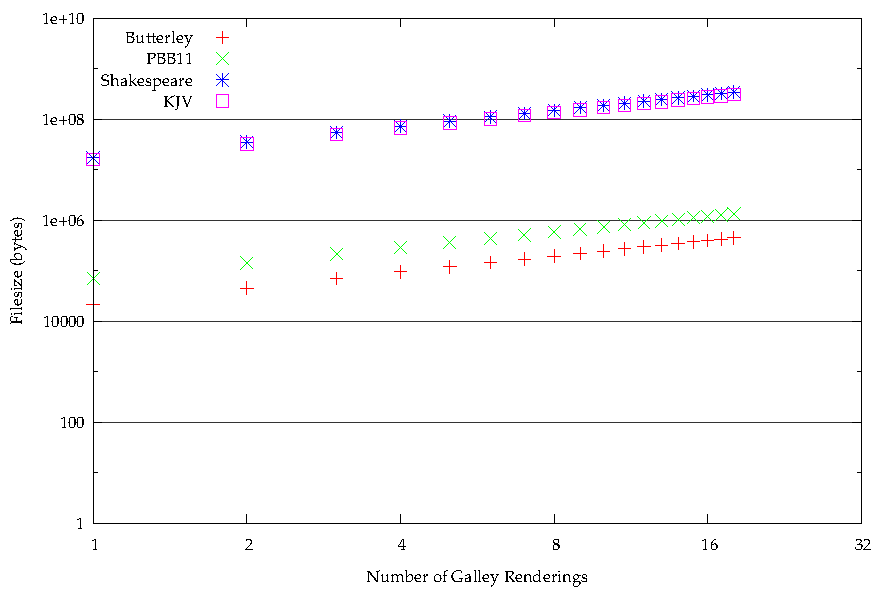
\includegraphics[width=\textwidth]{gnuplot/2-b}
  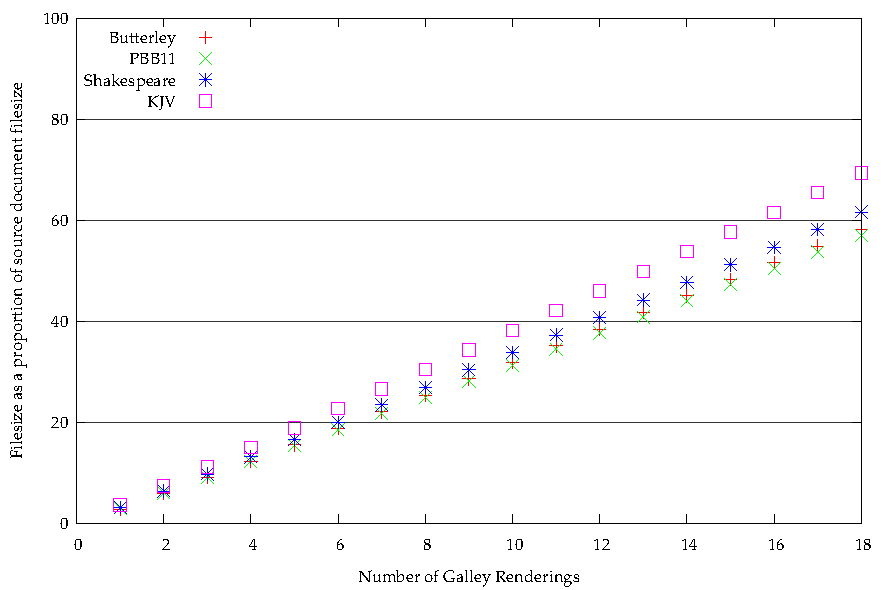
\includegraphics[width=\textwidth]{gnuplot/2-s}
  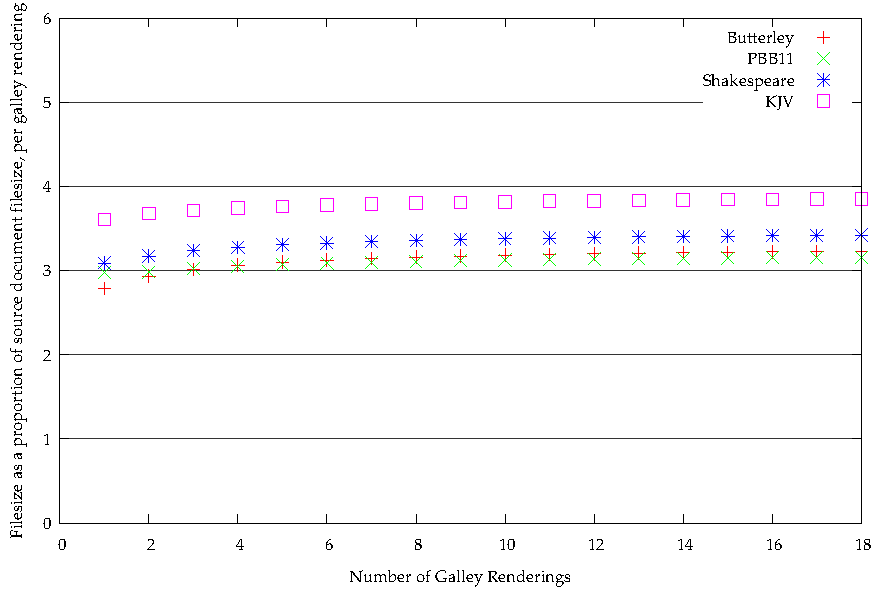
\includegraphics[width=\textwidth]{gnuplot/2-r}
  \end{center}
  \caption[Filesizes of documents in original encoding]{Filesizes of various documents, using the original encoding.}
  \label{fig:size-json}
\end{figure}



\begin{figure}
  \begin{center}
  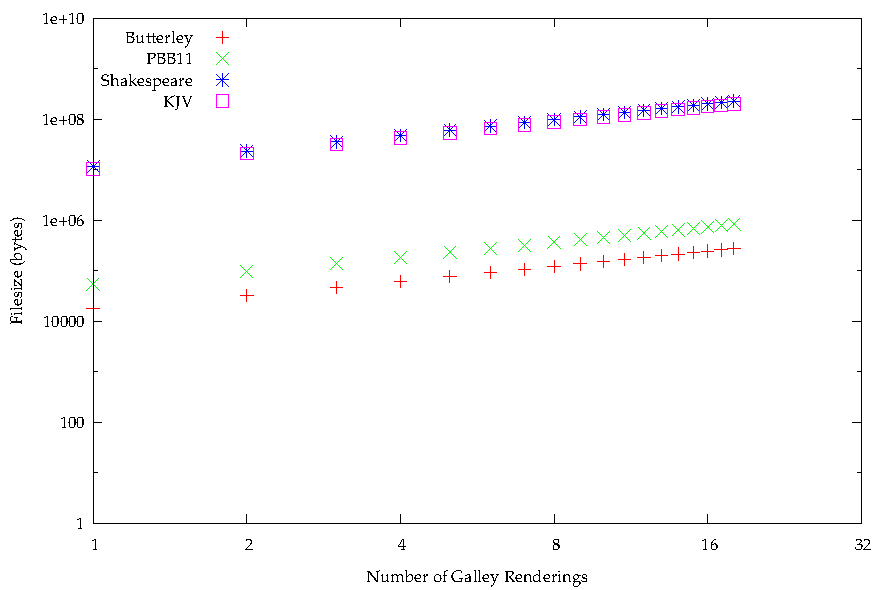
\includegraphics[width=\textwidth]{gnuplot/3-b}
  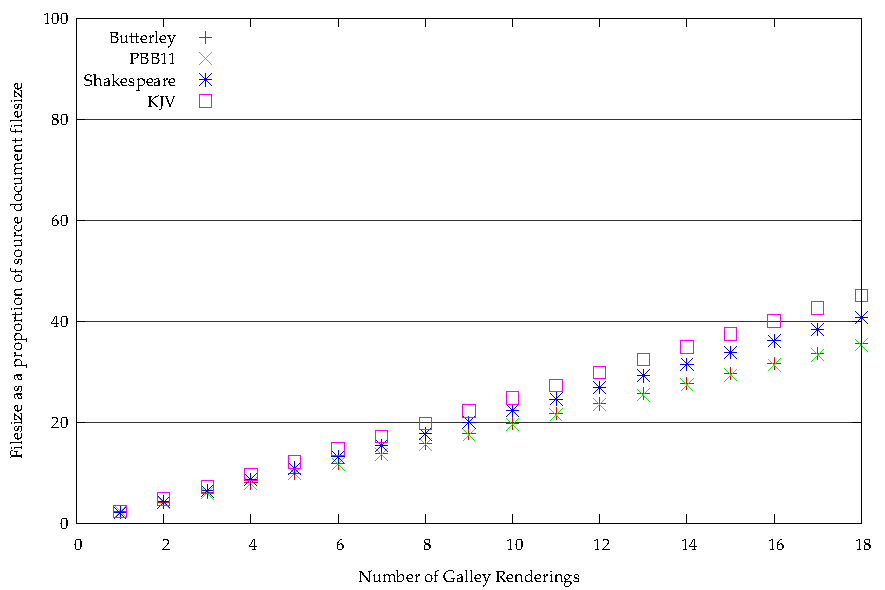
\includegraphics[width=\textwidth]{gnuplot/3-s}
  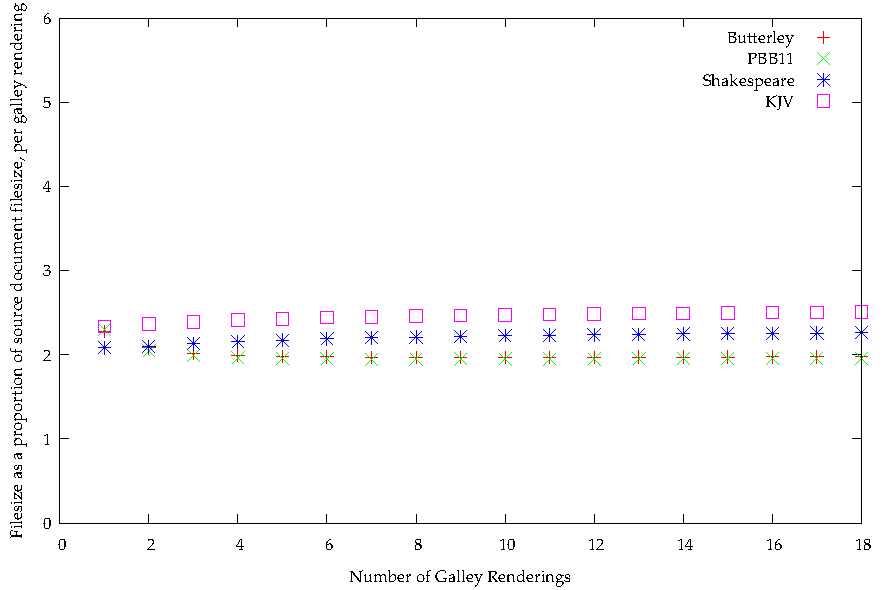
\includegraphics[width=\textwidth]{gnuplot/3-r}
  \end{center}
  \caption[Filesizes with an unordered dictionary]{Filesizes of various documents, encoded using an unordered dictionary.}
  \label{fig:size-unord}
\end{figure}



\begin{figure}
  \begin{center}
  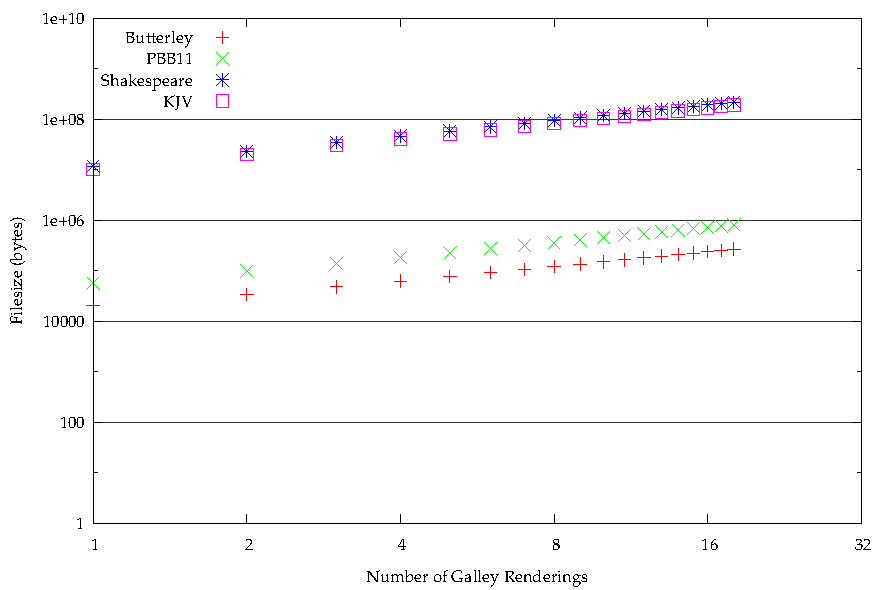
\includegraphics[width=\textwidth]{gnuplot/4-b}
  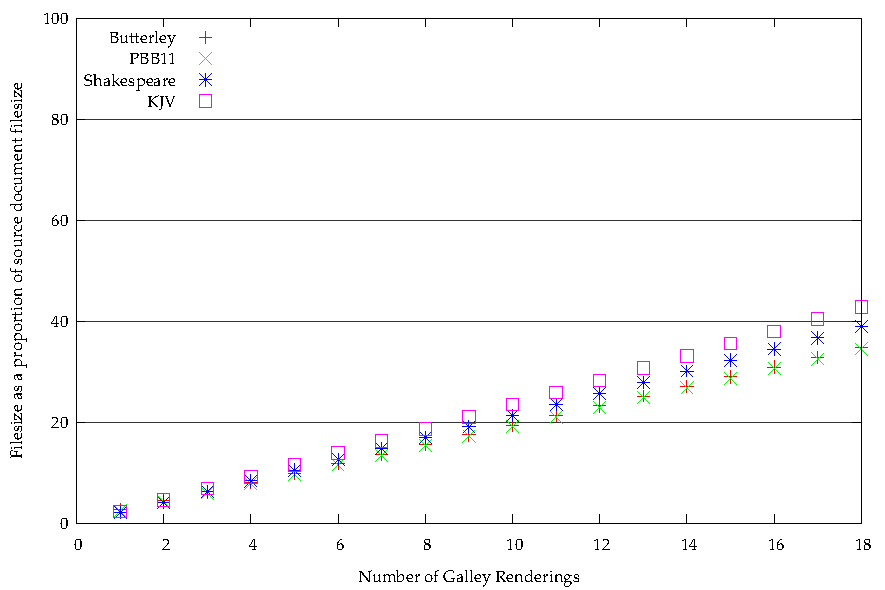
\includegraphics[width=\textwidth]{gnuplot/4-s}
  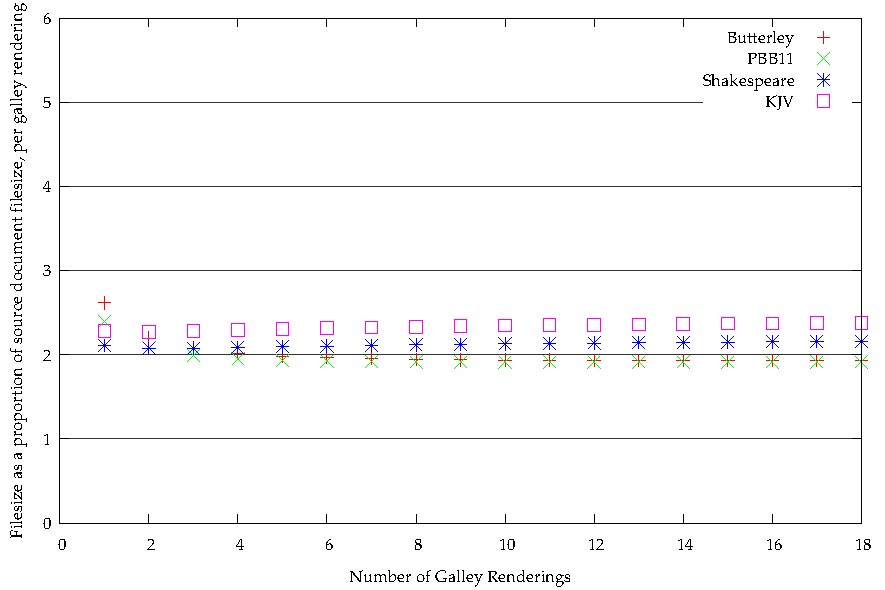
\includegraphics[width=\textwidth]{gnuplot/4-r}
  \end{center}
  \caption[Filesizes with an ordered dictionary]{Filesizes of various documents, encoded using an ordered dictionary.}
  \label{fig:size-ord}
\end{figure}



\begin{figure}
  \begin{center}
  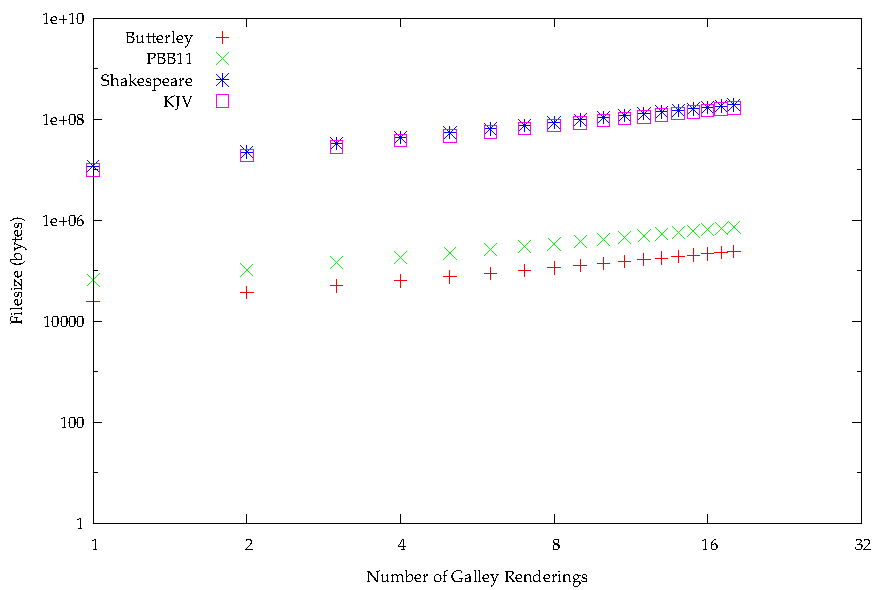
\includegraphics[width=\textwidth]{gnuplot/5-b}
  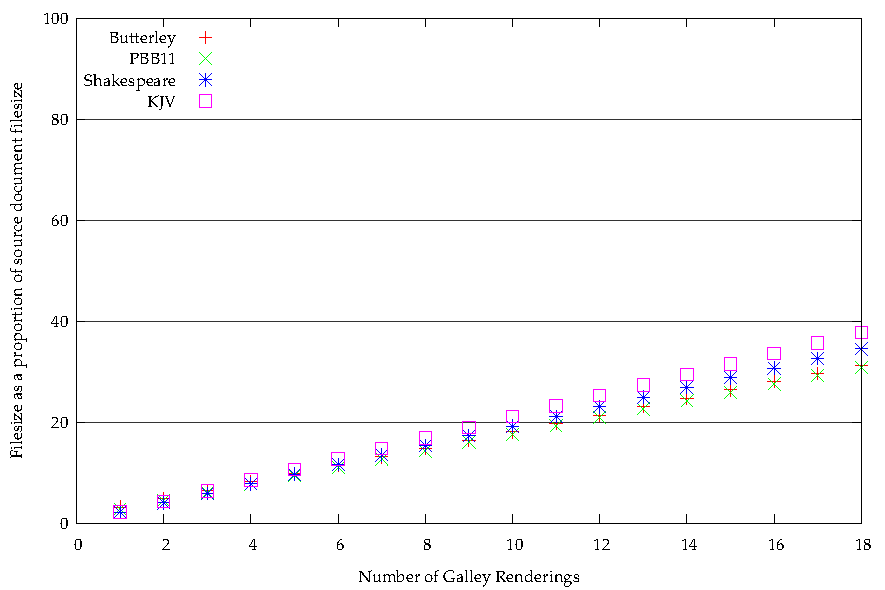
\includegraphics[width=\textwidth]{gnuplot/5-s}
  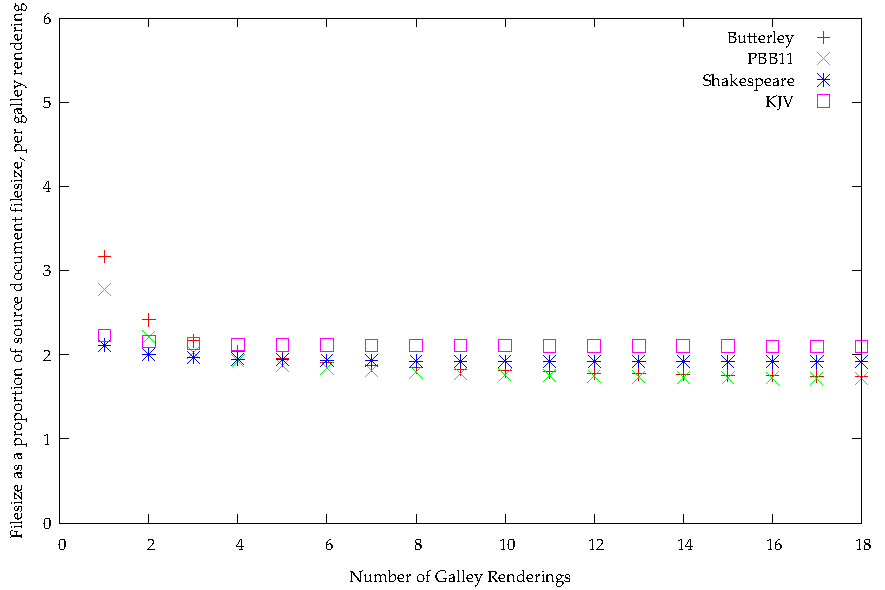
\includegraphics[width=\textwidth]{gnuplot/5-r}
  \end{center}
  \caption[Filesizes with relative positioning]{Filesizes of various documents, encoded using an ordered dictionary with word widths, and position deltas in the Galley Structure Tree.}
  \label{fig:size-deltas}
\end{figure}



\begin{figure}
  \begin{center}
  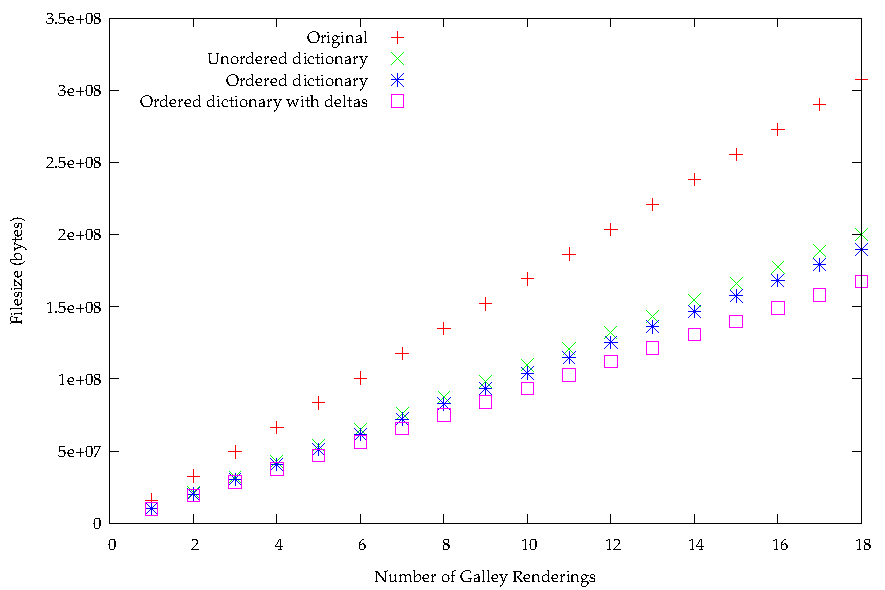
\includegraphics[height=\textwidth,angle=90]{gnuplot/kjv-b}
  \end{center}
  \caption[Comparison of filesizes from all encodings]{A comparison of filesizes produced by all encodings, using the King James Version of the Bible as a sample document.}
  \label{fig:size-all-b}
\end{figure}

\begin{figure}
  \begin{center}
  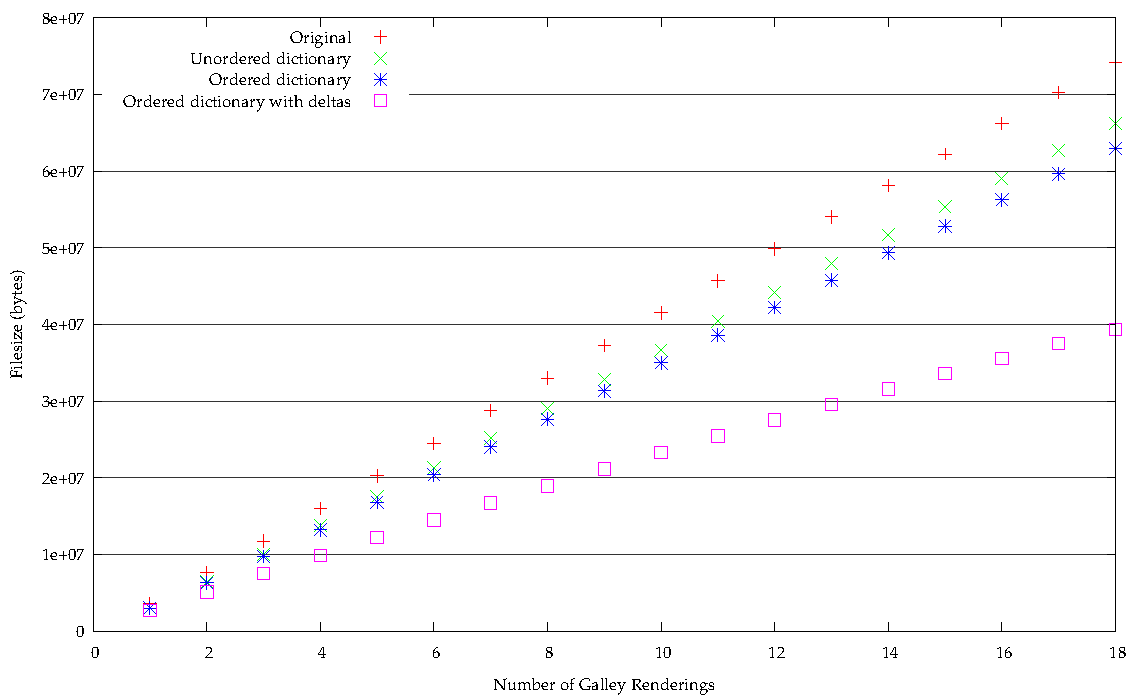
\includegraphics[height=\textwidth,angle=90]{gnuplot/kjv-gz}
  \end{center}
  \caption[Comparison of gzips of all encodings]{A comparison of filesizes of all encodings after gzipping, using the King James Version of the Bible as a sample document. Note the substantial improvement in compression of the encoding that uses position deltas over the variants that use absolute positioning.}
  \label{fig:size-all-gz}
\end{figure}


% \begin{table}
%     \myfloatalign
%   \begin{tabularx}{\textwidth}{lXXXXXX} %\toprule
%     & \multicolumn{2}{l}{\textsc{source text}} & \multicolumn{2}{l}{\textsc{orig. scheme}} & \multicolumn{2}{l}{\textsc{dictionary}} \\
%     & \textsc{plain} & \textsc{gz} & \textsc{plain} & \textsc{gz} & \textsc{plain} & \textsc{gz} \\ \midrule
%     PBB11~\cite{Pinkney2011} & 23\textsc{k} & 9.4\textsc{k} & 627\textsc{k} & 145\textsc{k} & 314\textsc{k} & 111\textsc{k} \\ \midrule
%     King James Bible & 4.3\textsc{m} & 1.4\textsc{m} & 144\textsc{m} & 32\textsc{m} & 73\textsc{m} & 24\textsc{m} \\ 
%     \bottomrule
%   \end{tabularx}
%   \caption[Comparison of filesizes]{Comparison of filesizes using various encoding methods}  \label{tab:filesize}
% \end{table}


\subsection{Discussion}

It is fairly clear from the above graphs that so long as some thought is put in, a lot of redundancy can be squeezed out of the data, without the need to resort to aggressive compression methods that require significant computation during decompression.

Nevertheless, Figures \ref{fig:size-all-b}~and~\ref{fig:size-all-gz} suggest that a significant amount of redundancy remains in each of the encoding schemes: on gzipping, the filesizes are reduced by some 66--75\%. Some of this can be attributed to \gls{json}'s syntax, but it is likely that the blame lies more with the data itself. The dictionary itself is not particularly compact. No advantage is taken of words that share common substrings, nor of words that have identical widths.

\todo{bleh}

\section{Summary}

